\newtcolorbox{textBox}[1][]{
	parbox=false,
	colback=Teal!10,
	colframe=Teal,
	colbacktitle=Teal,
	enhanced jigsaw,
	breakable,
	attach boxed title to top text left={yshift=-3mm,yshifttext=-3mm},
	#1,%
}


\section{``Nachhaltige'' Stadtplanung im 20. Jahrhundert}

\begin{myexercise}
	Lesen Sie einen der folgenden Texte und zeichnen Sie ein Modell der Stadt auf dem Flipchart auf. Präsentieren Sie das Modell sowie dessen Vor- und Nachteile der Klasse (ca. 3-4 Minuten).

	Aspekte Ihrer Präsentation:
	\begin{enumerate}
		\item Beweggründe für das Stadtmodell
		\item Schematischer Aufbau
		\item Mögliche Nachteile des Stadtmodells
		\item Inwiefern kann das Modell als ``nachhaltig'' bezeichnet werden?
		\item (Falls möglich: Reales Beispiel)
	\end{enumerate}
\end{myexercise}

\subsection{Die Gartenstadt}
\label{sec:gartenstadt}


\begin{textBox}[title=Die Gartenstadt]
	``Als Reaktion auf das unkontrollierte Städtewachstum sowie die schlechten Wohn- und Lebensbedingungen (als Folge der Industrialisierung in Grossbritannien) entwickelte der Brite Ebenezer Howard zu Beginn des 20. Jh. das städtebauliche Leitbild der Gartenstadt. Es war das erste Planungsmodell, das die städtischen Lebensbedingungen verbessern wollte. Es setzte weltweit Reformimpulse zukünftiger Stadt- und Raumplanung.

	Howards Ziel war die Errichtung mehrerer neuer, weitgehend autarker Gartenstädte mit einer begrenzten Einwohnerzahl, welche sich in einem gewissen Abstand von einer Grossstadt (Zentralstadt) befinden.

	Die Gartenstädte sollten durch einen Grüngürtel von der Zentralstadt getrennt sein. Als Verbindung sah er ein Verkehrsnetz aus radial angeordneten Strassen vor, die die Nachbarschaften entflechten und die Stadt in
	Segmente gliedern. In diesen konnten Doppelhäuser erbaut werden, welche von Garten- und Ackerland zur Selbstversorgung ebenso umgeben sind (Abb. \cref{fig:gartenstadt}).

	\begin{figure}[H]
		\centering
		\begin{subfigure}{.49\textwidth}
			\centering
			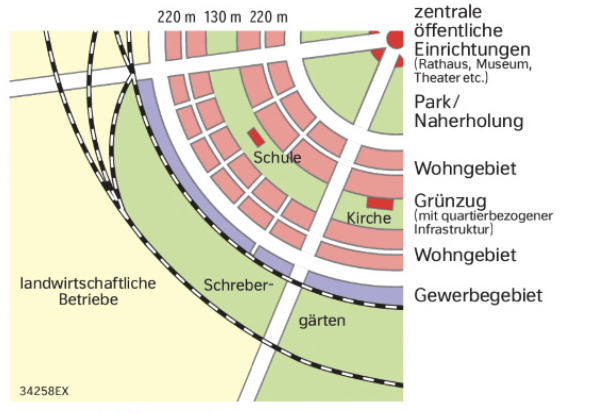
\includegraphics[width=\linewidth]{Geografie/Stadtgeografie/Figures/Stadtplanung/Gartenstadt-1}
			\caption{Räumliche Anordnung \cite{westermann}}
		\end{subfigure}
		\begin{subfigure}{.49\textwidth}
			\centering
			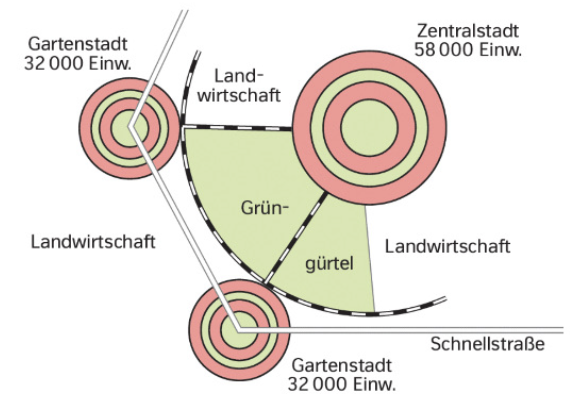
\includegraphics[width=\linewidth]{Geografie/Stadtgeografie/Figures/Stadtplanung/Gartenstadt-2}
			\caption{Teilplan der Gartenstadt\cite{westermann}}
		\end{subfigure}
		\caption{Die Gartenstadt von Howard \cite{westermann}}
		\label{fig:gartenstadt}
	\end{figure}

	Die Gartenstadt sollte sich auszeichnen durch eine geringe Bebauungsdichte, zentrale Einrichtungen (z. B.für Bildung und Kultur) sowie randlich gelegene Industrieareale, die durch Eisenbahnlinien und Kanäle verbunden sind. Auch die erforderlichen Arbeitsplätze für die Bewohner und zentrale Versorgungseinrichtungen sollten vorhanden sein, so dass keine grossen Pendlerwege entstehen würden. Dadurch käme es insgesamt zu einer aufgelockerten Stadt, mit dem Ziel, den Zuzug in die grossen [Zentral-]Städte zu bremsen und eine Dezentralisierung zu bewirken. Von den etwa einhundert geplanten Gartenstädten konnten lediglich zwei gebaut werden. Die bezweckte Dezentralisierung des Grosstadtwachstums wurde in Grossbritannien seit Mitte des 20. Jh. durch den Greater London Plan und durch die Errichtung zahlreicher „New Towns", die als Entlastungsstädte für London dienen sollten, verfolgt. Richtungsweisend für die heutige Zeit wurden sie wegen ihres Konzepts einer Stadtmitte, in der alle wichtigen Einrichtungen zur Befriedigung der Grundbedürfnisse zentriert sind. Die Gartenstadtidee hat den Städtebau in Mitteleuropa erheblich beeinflusst, z. B. bei der Errichtung von Werkskolonien oder bei der Anlage von gartenumgebenen Villen- oder Kleinhauskolonien in den Stadtrandzonen (s. \cref{fig:gartenstadt-3-kleinhauskolonie}).''

	--\textcite{westermann}

	\begin{figure}[H]
		\centering
		\includegraphics[width=0.5\linewidth]{"Geografie/Stadtgeografie/Figures/Stadtplanung/Gartenstadt-3-Kleinhauskolonie"}
		\caption{Kleinhauskolonie \cite{westermann}}
		\label{fig:gartenstadt-3-kleinhauskolonie}
	\end{figure}


\end{textBox}

\subsection{Die gegliederte Stadt}

\begin{textBox}[title=Die gegliederte Stadt]
	\textbf{Modelle kompakter Stadtanlagen für Grossstädte}

	``Wenige Jahrzehnte nach der Gartenstadtbewegung proklamierten Architekten und Stadtplaner, unter ihnen der Schweizer Le Corbusier, die Vorstellung, dass menschenwürdiges Wohnen nur durch einen radikalen Bruch mit der historischen Stadt zu erreichen sei. Mit dem Bau von Wohn-Hochhäusern („Wohn-Maschinen") wollte man hohe Einwohnerdichten im Kernbereich der Grossstadt erzielen (\textbf{vertikale Verdichtung}) und damit eine Konzentration von Einwohnern und
	Arbeitsplätzen auf engem Raum schaffen. Das Ziel war es, die ungehinderte Ausdehnung grosser Städte in das Umland zu begrenzen. Am Stadtrand zu errichtende Satellitenstädte sollten allein der Funktion des Wohnens dienen.
	Der utopische städtebauliche Plan von Le Corbusier zur Neugestaltung von Paris (\cref{fig:paris-corbusier}) konnte nicht
	verwirklicht werden. Seine und die Ideen anderer Architekten waren jedoch wegweisend für zukünftige Leitbilder und Modellvorstellungen.

	\begin{figure}[H]
		\centering
		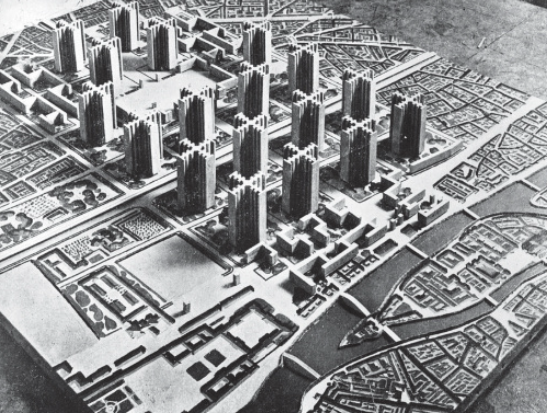
\includegraphics[width=0.5\linewidth]{Geografie/Stadtgeografie/Figures/Stadtplanung/paris-corbusier}
		\caption{Le Corbusiers Vision von Paris \cite{westermann}}
		\label{fig:paris-corbusier}
	\end{figure}

	\textbf{Modell der gegliederten und aufgelockerten Stadt}

	So verschieden die genannten Modellvorstellungen auch waren, gemeinsam war ihnen die Idee einer räumlichen Trennung von Arbeits- und Wohnstätten. Städteplaner aus ganz Europa gingen 1933 noch weiter. Sie bezogen in der \textbf{Charta von Athen} die Trennung der \textbf{Daseinsgrundfunktionen} nicht nur auf Arbeit und Wohnen, sondern auch auf Freizeit und Verkehr. Ihre Vorstellungen mündeten seit den 1950er-Jahren schliesslich in das generelle und bis in die Gegenwart wirkende Leitbild der \textbf{gegliederten und aufgelockerten Stadt} ein (\cref{fig:gegliederte-stadt}).

	\begin{figure}[H]
		\centering
		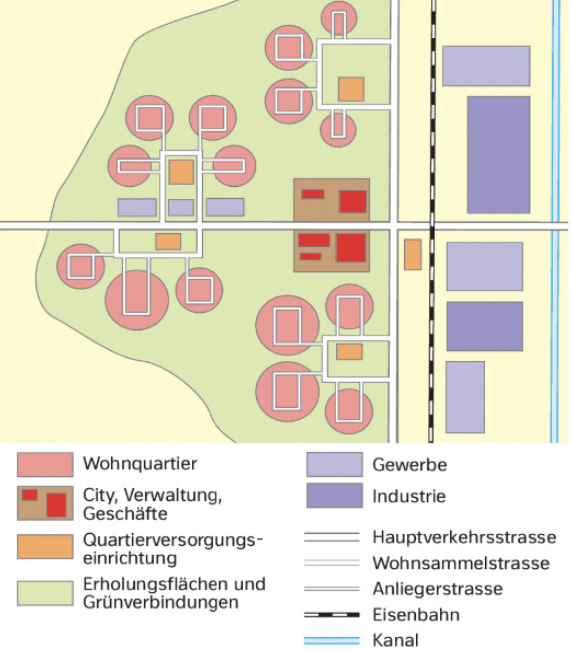
\includegraphics[width=0.5\linewidth]{Geografie/Stadtgeografie/Figures/Stadtplanung/gegliederte-Stadt}
		\caption{Struktur der gegliederten und aufgelockerten Stadt \cite{westermann}}
		\label{fig:gegliederte-stadt}
	\end{figure}

	In der Realität jedoch mussten sich die Städte in den Staaten des Westens in erster Linie auf den beschleunigten ökonomischen und sozialen Wandel und die steigende Mobilität der Bevölkerung einstellen. Der Fokus der Stadtentwicklung wechselte dabei rascher als jemals zuvor, pendelte zwischen Innenstadt, Innenstadtrand und Aussenbereichen. Vielerorts gab es kurz- oder mittelfristig gerade noch realisierbare Teillösungen für Stadt oder Umland. So musste man z. B. auf den dramatischen Nutzungswandel im Stadtkern, den Zerfall der innenstadtnahen Misch- und Gewerbegebiete, den Wegzug von Bevölkerung ins Umland (\textbf{Suburbanisierung}) und damit einhergehende wachsende Pendlerströme reagieren.[...]

	\textbf{[Zusammenfassung:]} Le Corbusiers Konzept und ebenso die Gartenstadtbewegung gaben den Anstoss für das Leitbild der \textbf{gegliederten und aufgelockerten Stadt} (\cref{fig:gegliederte-stadt}), das seit den 1950er-Jahren zur bestimmenden stadtplanerischen Strömung wurde. Dieses Leitbild sah eine in einzelne Siedlungs- und Nutzungsbereiche gegliederte, durch Grünzüge aufgelockerte und mit Naherholungsflächen verbundene Stadt vor. Durch die Entwicklung der schienengebundenen Verkehrsmittel und des motorisierten Verkehrs war es dann seit den 1950er-Jahren möglich geworden, die einzelnen Funktionszonen mehr und mehr zu trennen. Besonders das Auto wurde zum vermittelnden Medium in der gegliederten Stadtlandschaft.''

	--\textcite{westermann}

\end{textBox}

\subsection{Die Stadt der kurzen Wege}

\begin{textBox}[title=Stadt der kurzen Wege]
	``Seit den 1960er-Jahren war Stadtplanung in erster Linie Verkehrsplanung. Gemäss dem Leitbild der \textbf{autogerechten Stadt} sollten sich die Planungsmassnahmen dem ungehinderten Verkehrsfluss des Autos unterordnen. Dies führte zu einer flächenfressenden Siedlungsexpansion (\textbf{Suburbanisierung}) und zu einer \textbf{Zersiedelung} der Landschaft (\cref{fig:stadtplanung}). Durch die zunehmende Mobilität der Bevölkerung konnte mehr gependelt werden, Verkehrs- und Umweltbelastungen stiegen stetig an.

	In den 1970er-Jahren formierten sich Widerstände gegen das Leitbild der autogerechten Stadt. Die sich zuspitzende Umweltdiskussion hielt Einzug in die Stadtplanung. So sollten auch ökologische Fragestellungen stärker in die Stadtplanung mit einfliessen. Aus diesem Ansatz heraus entstand seit der UN-Konferenz für Umwelt und Entwicklung in Rio de Janeiro (1992) und den dadurch eingeleiteten lokalen Handlungsprogrammen (Lokale Agenda 21) das Leitbild der nachhaltigen Stadtentwicklung. Ein wichtiger Aspekt dabei ist unter anderem, dass die Daseinsgrundfunktionen wieder vermehrt an einem Ort durchmischt werden sollen. Durch eine Stadt der kurzen Wege liessen sich unnötiges Pendeln und der Verkehr allgemein minimieren.''

	--\textcite{westermann}

	\begin{quotation}
		Als räumliche Ordnungsprinzipien der nachhaltigen Stadtentwicklung (...) werden seit den
		1990er-Jahren u.a. drei Punkte diskutiert:

		\begin{enumerate}
			\item  \textbf{Dichte im Städtebau}, d.h. die Schaffung kompakterer und hochwertiger baulicher Strukturen, die ein Ausufern der Siedlungen in die Fläche verhindern sollen. (...)
			\item  \textbf{Nutzungsmischung}, (...) d.h. die funktionale Mischung innerhalb von Stadtquartieren durch
			      Verflechtungen von Wohnen und Arbeiten, aber auch von Versorgung und Freizeit. (...) Von Bedeutung sind auch die Förderung sozialer Mischungen nach Einkommensklassen, Haushaltstypen und Lebensstilgruppen sowie die Planung baulicher Mischungen.
			\item (...) die sog. \textbf{Polyzentralität}, insbesondere in
			      Gestalt der sog. dezentralen Konzentration (...).
			      (...) Dadurch können der anhaltende Siedlungsdruck im Umland der Städte auf ausgewählte Siedlungsschwerpunkte gebündelt und etwa auch eine grössere Tragfähigkeit des ÖPNV (öffentlicher Nahverkehrs) erreicht werden.
		\end{enumerate}
		(Quelle: Heinz Heineberg: Stadtgeographie. Schöningh, UTB.
		Paderbom. 2006, S. 142 - 144)
	\end{quotation}
	\begin{figure}[H]
		\centering
		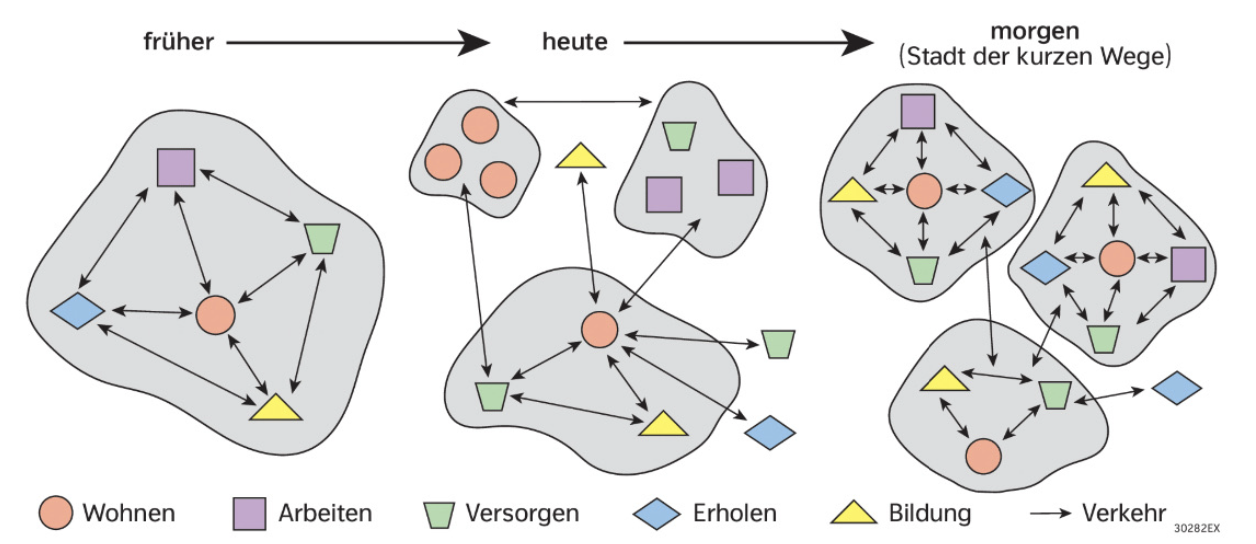
\includegraphics[width=\linewidth]{Geografie/Stadtgeografie/Figures/Stadtplanung/Stadtplanung}
		\caption{Modell der Entwicklung der räumlichen Muster der Daseinsgrundfunktionen bis zu einer ``Stadt der kurzen Wege'' \cite{westermann}}
		\label{fig:stadtplanung}
	\end{figure}
\end{textBox}

\subsection{Gemeinsamkeiten nachhaltiger Verkehrsplanung im 20. Jahrhundert}
\notiz{8}

\section{Nachhaltige Stadtplanung im 21. Jahrhundert}

\begin{myexercise}[Placemat zu nachhaltiger Stadtplanung]
	Informieren Sie sich anhand des Ihnen zugeteilten Artikels über Projekte zur Umsetzung nachhaltiger Stadtplanung.

	Halten Sie Ihre individuellen Antworten auf folgende Fragen auf dem Placemat fest:

	\begin{itemize}
		\item Wie hat sich die präsentierte Stadt verändert?
		\item Aus welchen Gründen hat sie sich verändert?
		\item Welche Herausforderungen stellen sich?
		\item Ginge das auch in der Schweiz? Weshalb (nicht)?
	\end{itemize}

	Gleichen Sie danach Ihre Antworten ab und halten Sie die wichtigsten Aspekte im mittleren Feld des Placemats fest.

	Präsentieren Sie danach den zentralen Teil Ihres Placemats kurz der Klasse.

\end{myexercise}

\begin{textBox}[title=Paris]
	\begin{figure}[H]
		\centering
		\colorbox{white}{
\includegraphics[width=.8\linewidth]{"Geografie/Stadtgeografie/NZZ-Artikel/Seite_8_NZZ_-_Neue_Zürcher_Zeitung_2024-08-30.pdf"}}
		%\caption{NZZ-Artikel zu Paris}
		%\label{fig:seite8nzz-neuezurcherzeitung2024-08-30}
	\end{figure}
\end{textBox}

\begin{textBox}[title=Singapur]
	\begin{figure}[H]
		\centering
		\colorbox{white}{
\includegraphics[width=.8\linewidth]{"Geografie/Stadtgeografie/NZZ-Artikel/Seite_15_NZZ_-_Neue_Zürcher_Zeitung_2023-08-26.pdf"}}
		%\caption{NZZ-Artikel zu Singapur}
	\end{figure}
\end{textBox}

\begin{textBox}[title=Dubai]
	\begin{figure}[H]
		\centering
		\colorbox{white}{
\includegraphics[width=.8\linewidth, page=2]{"Geografie/Stadtgeografie/NZZ-Artikel/Seiten_48_49_NZZ_-_Neue_Zürcher_Zeitung_2023-06-24.pdf"}}
		%\caption{NZZ-Artikel zu Dubai}
	\end{figure}

\end{textBox}

\begin{textBox}[title=Schweiz]
	\begin{figure}[H]
		\centering
		\colorbox{white}{
\includegraphics[width=.8\linewidth, page=1]{"Geografie/Stadtgeografie/NZZ-Artikel/Seiten_10_11_NZZ_-_Neue_Zürcher_Zeitung_2022-05-09.pdf"}}

	\end{figure}
	\begin{figure}[H]
		\centering
		\colorbox{white}{
\includegraphics[width=.8\linewidth, page=2]{"Geografie/Stadtgeografie/NZZ-Artikel/Seiten_10_11_NZZ_-_Neue_Zürcher_Zeitung_2022-05-09.pdf"}}
	\end{figure}
\end{textBox}

\section{Lernziele}
\begin{todolist}
	\item Ich kann wichtige Stadtplanungs-Konzepte aus dem 20. Jahrhundert benennen und charakterisieren, insbesondere \textit{die Gartenstadt}, \textit{die aufgelockerte Stadt} und \textit{die Stadt der kurzen Wege}.
	\item Ich kann für folgende Stadtmodelle eine schematische Darstellung aufzeichnen sowie Vor- sowie Nachteile erläutern: \textit{Die Gartenstadt}, \textit{die aufgelockerte Stadt} und die \textit{Stadt der kurzen Wege}.
	\item Ich kann Gemeinsamkeiten nachhaltiger Stadt-Modelle im 20. Jahrhundert benennen und beschreiben (Begrünung, Verdichtung, Verkehrsmanagement)
	\item Ich kann Tendenzen gegenwärtiger, nachhaltiger Stadt-Verkehrsplanung im In- und Ausland benennen.
	\item Ich kann Massnahmen, um das Konzept der \textit{Netto-Null-Stadt} zu erreichen, benennen und hinsichtlich deren Effektivität bewerten.
\end{todolist}
